% Options for packages loaded elsewhere
\PassOptionsToPackage{unicode}{hyperref}
\PassOptionsToPackage{hyphens}{url}
%
\documentclass[
]{article}
\usepackage{lmodern}
\usepackage{amssymb,amsmath}
\usepackage{ifxetex,ifluatex}
\ifnum 0\ifxetex 1\fi\ifluatex 1\fi=0 % if pdftex
  \usepackage[T1]{fontenc}
  \usepackage[utf8]{inputenc}
  \usepackage{textcomp} % provide euro and other symbols
\else % if luatex or xetex
  \usepackage{unicode-math}
  \defaultfontfeatures{Scale=MatchLowercase}
  \defaultfontfeatures[\rmfamily]{Ligatures=TeX,Scale=1}
\fi
% Use upquote if available, for straight quotes in verbatim environments
\IfFileExists{upquote.sty}{\usepackage{upquote}}{}
\IfFileExists{microtype.sty}{% use microtype if available
  \usepackage[]{microtype}
  \UseMicrotypeSet[protrusion]{basicmath} % disable protrusion for tt fonts
}{}
\makeatletter
\@ifundefined{KOMAClassName}{% if non-KOMA class
  \IfFileExists{parskip.sty}{%
    \usepackage{parskip}
  }{% else
    \setlength{\parindent}{0pt}
    \setlength{\parskip}{6pt plus 2pt minus 1pt}}
}{% if KOMA class
  \KOMAoptions{parskip=half}}
\makeatother
\usepackage{xcolor}
\IfFileExists{xurl.sty}{\usepackage{xurl}}{} % add URL line breaks if available
\IfFileExists{bookmark.sty}{\usepackage{bookmark}}{\usepackage{hyperref}}
\hypersetup{
  hidelinks,
  pdfcreator={LaTeX via pandoc}}
\urlstyle{same} % disable monospaced font for URLs
\usepackage[margin=1in]{geometry}
\usepackage{longtable,booktabs}
% Correct order of tables after \paragraph or \subparagraph
\usepackage{etoolbox}
\makeatletter
\patchcmd\longtable{\par}{\if@noskipsec\mbox{}\fi\par}{}{}
\makeatother
% Allow footnotes in longtable head/foot
\IfFileExists{footnotehyper.sty}{\usepackage{footnotehyper}}{\usepackage{footnote}}
\makesavenoteenv{longtable}
\usepackage{graphicx}
\makeatletter
\def\maxwidth{\ifdim\Gin@nat@width>\linewidth\linewidth\else\Gin@nat@width\fi}
\def\maxheight{\ifdim\Gin@nat@height>\textheight\textheight\else\Gin@nat@height\fi}
\makeatother
% Scale images if necessary, so that they will not overflow the page
% margins by default, and it is still possible to overwrite the defaults
% using explicit options in \includegraphics[width, height, ...]{}
\setkeys{Gin}{width=\maxwidth,height=\maxheight,keepaspectratio}
% Set default figure placement to htbp
\makeatletter
\def\fps@figure{htbp}
\makeatother
\setlength{\emergencystretch}{3em} % prevent overfull lines
\providecommand{\tightlist}{%
  \setlength{\itemsep}{0pt}\setlength{\parskip}{0pt}}
\setcounter{secnumdepth}{5}
\usepackage{caption} \captionsetup{font={footnotesize},width=6in} \renewcommand{\dblfloatpagefraction}{.9} \makeatletter \renewenvironment{figure} {\def\@captype{figure}} \makeatother \@ifundefined{Shaded}{\newenvironment{Shaded}} \@ifundefined{snugshade}{\newenvironment{snugshade}} \renewenvironment{Shaded}{\begin{snugshade}}{\end{snugshade}} \definecolor{shadecolor}{RGB}{230,230,230} \usepackage{xeCJK} \usepackage{setspace} \setstretch{1.3} \usepackage{tcolorbox} \setcounter{secnumdepth}{4} \setcounter{tocdepth}{4} \usepackage{wallpaper} \usepackage[absolute]{textpos} \tcbuselibrary{breakable} \renewenvironment{Shaded} {\begin{tcolorbox}[colback = gray!10, colframe = gray!40, width = 16cm, arc = 1mm, auto outer arc, title = {R input}]} {\end{tcolorbox}} \usepackage{titlesec} \titleformat{\paragraph} {\fontsize{10pt}{0pt}\bfseries} {\arabic{section}.\arabic{subsection}.\arabic{subsubsection}.\arabic{paragraph}} {1em} {} []
\newlength{\cslhangindent}
\setlength{\cslhangindent}{1.5em}
\newenvironment{cslreferences}%
  {}%
  {\par}

\author{}
\date{\vspace{-2.5em}}

\begin{document}

\begin{titlepage} \newgeometry{top=7.5cm}
\ThisCenterWallPaper{1.12}{~/outline/lixiao//cover_page.pdf}
\begin{center} \textbf{\Huge
筛选差异蛋白和对应配体蛋白} \vspace{4em}
\begin{textblock}{10}(3,5.9) \huge
\textbf{\textcolor{white}{2024-03-08}}
\end{textblock} \begin{textblock}{10}(3,7.3)
\Large \textcolor{black}{LiChuang Huang}
\end{textblock} \begin{textblock}{10}(3,11.3)
\Large \textcolor{black}{@立效研究院}
\end{textblock} \end{center} \end{titlepage}
\restoregeometry

\pagenumbering{roman}

\tableofcontents

\listoffigures

\listoftables

\newpage

\pagenumbering{arabic}

\hypertarget{abstract}{%
\section{摘要}\label{abstract}}

\begin{itemize}
\tightlist
\item
  研究对象:乳腺癌或结直肠癌
\item
  耐药:5-氟尿嘧啶或顺铂
\end{itemize}

\hypertarget{ux9700ux6c42}{%
\subsection{需求}\label{ux9700ux6c42}}

1、寻找差异致癌膜蛋白及对应配体蛋白;
2、耐药差异膜蛋白及对应抗体蛋白或互作抑制其表达蛋白。

现需要利用数据库分析正常组与疾病组间的差异表达膜蛋白AA(在癌中高表达的)和对应靶向癌细胞特异性高表达的膜蛋白AA的配体蛋白AA';
以及非耐药组与耐药组间的差异表达膜蛋白XX(在耐药组中高表达的)和对应XX的抗体蛋白或相互作用能抑制其表达的蛋白XX'。

\hypertarget{ux7ed3ux679c}{%
\subsection{结果}\label{ux7ed3ux679c}}

\hypertarget{ux5bfbux627eux5deeux5f02ux81f4ux764cux819cux86cbux767dux53caux5bf9ux5e94ux914dux4f53ux86cbux767d}{%
\subsubsection{寻找差异致癌膜蛋白及对应配体蛋白}\label{ux5bfbux627eux5deeux5f02ux81f4ux764cux819cux86cbux767dux53caux5bf9ux5e94ux914dux4f53ux86cbux767d}}

这一部分思路较简单,找到可用的蛋白质组数据\textsuperscript{\protect\hyperlink{ref-ProteomicsProfShao2022}{1}},筛选差异蛋白,
再以 UniTmp 数据库筛选跨膜蛋白 (膜蛋白受体主要为跨膜蛋白) ,再借助 STRINGdb 构建
PPI 网络,寻找互作蛋白,再结合富集分析 (\ref{cut-ppi}),进一步缩小范围。

注意,以上 PPI 构建的来源是所有筛选到的差异蛋白 (拟从差异蛋白中找到候选的配体蛋白)。

差异癌膜蛋白为:AIFM1, TFRC, ITGAM, PECAM1
最终筛选的蛋白和对应候选配体关系见:Fig. \ref{fig:PPS-DPS-filtered-by-KEGG-and-formated-PPI-network}

\hypertarget{ux8010ux836fux5deeux5f02ux819cux86cbux767dux53caux5bf9ux5e94ux6297ux4f53ux86cbux767dux6216ux4e92ux4f5cux6291ux5236ux5176ux8868ux8fbeux86cbux767d}{%
\subsubsection{耐药差异膜蛋白及对应抗体蛋白或互作抑制其表达蛋白}\label{ux8010ux836fux5deeux5f02ux819cux86cbux767dux53caux5bf9ux5e94ux6297ux4f53ux86cbux767dux6216ux4e92ux4f5cux6291ux5236ux5176ux8868ux8fbeux86cbux767d}}

这部分思路稍复杂。由于无法直接获得包含耐药性分组的蛋白表达数据,因此需要另寻思路,
即,获取 TCGA-COAD 的基因表达数据和蛋白定量数据,以 \texttt{pRRophetic} 根据基因表达数据
分析耐药性 (顺铂 Cisplatin),再对样本分组,随后分析蛋白定量数据。

后续和上一部分近似:筛选差异蛋白,再以 UniTmp 数据库筛选跨膜蛋白,再借助 STRINGdb 构建
PPI 网络,寻找互作蛋白,再结合富集分析。到这里,筛选蛋白 (TSC1) 和互作蛋白关系见
Fig. \ref{fig:TCGA-DPS-filtered-and-formated-PPI-network-logFC}。
后续的富集分析结果可能有一定参考价值,富集到 TSC1
(hsa04151, Fig. \ref{fig:TCGA-TSC1-in-hsa04151-visualization})

注意,以上 PPI 构建的来源是筛选的膜蛋白 (TSC1),和 RNA-seq 的 DEGs (拟从差异蛋白中找到候选的配体蛋白)。

但这部分还需要指定互作抑制的蛋白,因此又结合了关联分析,挖掘 RNA 表达中呈负相关性的蛋白
(Fig. \ref{fig:TCGA-RNA-correlation-heatmap})。

最终可参考的表格:Tab. \ref{tab:TCGA-RNA-TSC1-negtive-correlated}

\hypertarget{introduction}{%
\section{前言}\label{introduction}}

\hypertarget{methods}{%
\section{材料和方法}\label{methods}}

\hypertarget{ux6750ux6599}{%
\subsection{材料}\label{ux6750ux6599}}

Other data obtained from published article (e.g., supplementary tables):

\begin{itemize}
\tightlist
\item
  Supplementary file from article refer to\textsuperscript{\protect\hyperlink{ref-ProteomicsProfShao2022}{1}}.
\end{itemize}

\hypertarget{ux65b9ux6cd5}{%
\subsection{方法}\label{ux65b9ux6cd5}}

Mainly used method:

\begin{itemize}
\tightlist
\item
  R package \texttt{ClusterProfiler} used for gene enrichment analysis\textsuperscript{\protect\hyperlink{ref-ClusterprofilerWuTi2021}{2}}.
\item
  R package \texttt{Limma} and \texttt{edgeR} used for differential expression analysis\textsuperscript{\protect\hyperlink{ref-LimmaPowersDiRitchi2015}{3},\protect\hyperlink{ref-EdgerDifferenChen}{4}}.
\item
  R Package \texttt{pRRophetic} was used for Prediction of Clinical Chemotherapeutic Response\textsuperscript{\protect\hyperlink{ref-PrropheticAnGeeleh2014}{5}}.
\item
  R package \texttt{STEINGdb} used for PPI network construction\textsuperscript{\protect\hyperlink{ref-TheStringDataSzklar2021}{6},\protect\hyperlink{ref-CytohubbaIdenChin2014}{7}}.
\item
  R package \texttt{TCGAbiolinks} used for abtain TCGA dataset\textsuperscript{\protect\hyperlink{ref-TcgabiolinksAColapr2015}{8}}.
\item
  The UNIfied database of TransMembrane Proteins (UniTmp) was used for transmembrane protein information retrieving\textsuperscript{\protect\hyperlink{ref-UnitmpUnifiedDobson2024}{9},\protect\hyperlink{ref-TheHumanTransDobson2015}{10}}.
\item
  The MCC score was calculated referring to algorithm of \texttt{CytoHubba}\textsuperscript{\protect\hyperlink{ref-CytohubbaIdenChin2014}{7}}.
\item
  R version 4.3.2 (2023-10-31); Other R packages (eg., \texttt{dplyr} and \texttt{ggplot2}) used for statistic analysis or data visualization.
\end{itemize}

\hypertarget{results}{%
\section{分析结果}\label{results}}

\hypertarget{dis}{%
\section{结论}\label{dis}}

\hypertarget{workflow1}{%
\section{附:分析流程------寻找差异致癌膜蛋白及对应配体蛋白}\label{workflow1}}

\hypertarget{ux7ed3ux76f4ux80a0ux764cux5deeux5f02ux86cbux767d}{%
\subsection{结直肠癌差异蛋白}\label{ux7ed3ux76f4ux80a0ux764cux5deeux5f02ux86cbux767d}}

\hypertarget{ux6570ux636eux6765ux6e90}{%
\subsubsection{数据来源}\label{ux6570ux636eux6765ux6e90}}

Proteomics profiling of colorectal cancer progression identifies PLOD2 as a potential therapeutic target\textsuperscript{\protect\hyperlink{ref-ProteomicsProfShao2022}{1}}

Table \ref{tab:PUBLISHED-ProteomicsProfShao2022-metadata-used-sample} (下方表格) 为表格PUBLISHED ProteomicsProfShao2022 metadata used sample概览。

\textbf{(对应文件为 \texttt{Figure+Table/PUBLISHED-ProteomicsProfShao2022-metadata-used-sample.csv})}

\begin{center}\begin{tcolorbox}[colback=gray!10, colframe=gray!50, width=0.9\linewidth, arc=1mm, boxrule=0.5pt]注:表格共有31行5列,以下预览的表格可能省略部分数据;表格含有2个唯一`group'。
\end{tcolorbox}
\end{center}
\begin{center}\begin{tcolorbox}[colback=gray!10, colframe=gray!50, width=0.9\linewidth, arc=1mm, boxrule=0.5pt]\begin{enumerate}\tightlist
\item sample:  样品名称
\item group:  分组名称
\end{enumerate}\end{tcolorbox}
\end{center}

\begin{longtable}[]{@{}lllll@{}}
\caption{\label{tab:PUBLISHED-ProteomicsProfShao2022-metadata-used-sample}PUBLISHED ProteomicsProfShao2022 metadata used sample}\tabularnewline
\toprule
sample & Gender & Age & Pathology.Type & group\tabularnewline
\midrule
\endfirsthead
\toprule
sample & Gender & Age & Pathology.Type & group\tabularnewline
\midrule
\endhead
P1 & Female & 74 & Normal Colon & Control\tabularnewline
P2 & Female & 49 & Normal Colon & Control\tabularnewline
P5 & Male & 51 & Normal Colon & Control\tabularnewline
P6 & Female & 56 & Normal Colon & Control\tabularnewline
P7 & Male & 53 & Normal Colon & Control\tabularnewline
P8 & Male & 70 & Normal Colon & Control\tabularnewline
P9 & Male & 62 & Normal Colon & Control\tabularnewline
P11 & Male & 48 & Normal Colon & Control\tabularnewline
P13 & Female & 43 & Normal Colon & Control\tabularnewline
P14 & Female & 61 & Normal Colon & Control\tabularnewline
P15 & Female & 81 & Normal Colon & Control\tabularnewline
P16 & Male & 67 & Normal Colon & Control\tabularnewline
P17 & Male & 60 & Normal Colon & Control\tabularnewline
P18 & Female & 59 & Normal Colon & Control\tabularnewline
P19 & Male & 64 & Normal Colon & Control\tabularnewline
\ldots{} & \ldots{} & \ldots{} & \ldots{} & \ldots{}\tabularnewline
\bottomrule
\end{longtable}

\hypertarget{ux5deeux5f02ux86cbux767d}{%
\subsubsection{差异蛋白}\label{ux5deeux5f02ux86cbux767d}}

Figure \ref{fig:PPS-Cancer-vs-Control-DEGs} (下方图) 为图PPS Cancer vs Control DEGs概览。

\textbf{(对应文件为 \texttt{Figure+Table/PPS-Cancer-vs-Control-DEGs.pdf})}

\def\@captype{figure}
\begin{center}
\includegraphics[width = 0.9\linewidth]{Figure+Table/PPS-Cancer-vs-Control-DEGs.pdf}
\caption{PPS Cancer vs Control DEGs}\label{fig:PPS-Cancer-vs-Control-DEGs}
\end{center}

Table \ref{tab:PPS-data-Cancer-vs-Control-DPs} (下方表格) 为表格PPS data Cancer vs Control DPs概览。

\textbf{(对应文件为 \texttt{Figure+Table/PPS-data-Cancer-vs-Control-DPs.csv})}

\begin{center}\begin{tcolorbox}[colback=gray!10, colframe=gray!50, width=0.9\linewidth, arc=1mm, boxrule=0.5pt]注:表格共有509行8列,以下预览的表格可能省略部分数据;表格含有509个唯一`Gene\_name'。
\end{tcolorbox}
\end{center}
\begin{center}\begin{tcolorbox}[colback=gray!10, colframe=gray!50, width=0.9\linewidth, arc=1mm, boxrule=0.5pt]\begin{enumerate}\tightlist
\item logFC:  estimate of the log2-fold-change corresponding to the effect or contrast (for ‘topTableF’ there may be several columns of log-fold-changes)
\item AveExpr:  average log2-expression for the probe over all arrays and channels, same as ‘Amean’ in the ‘MarrayLM’ object
\item t:  moderated t-statistic (omitted for ‘topTableF’)
\item P.Value:  raw p-value
\item B:  log-odds that the gene is differentially expressed (omitted for ‘topTreat’)
\end{enumerate}\end{tcolorbox}
\end{center}

\begin{longtable}[]{@{}llllllll@{}}
\caption{\label{tab:PPS-data-Cancer-vs-Control-DPs}PPS data Cancer vs Control DPs}\tabularnewline
\toprule
Gene\_name & logFC & rownames & AveExpr & t & P.Value & adj.P.Val & B\tabularnewline
\midrule
\endfirsthead
\toprule
Gene\_name & logFC & rownames & AveExpr & t & P.Value & adj.P.Val & B\tabularnewline
\midrule
\endhead
EFEMP1 & 2.2381\ldots{} & Q12805 & 5.4470\ldots{} & 8.2464\ldots{} & 3.7745\ldots{} & 1.8231\ldots{} & 10.666\ldots{}\tabularnewline
P4HA1 & 2.2015\ldots{} & P13674 & 4.8852\ldots{} & 6.6539\ldots{} & 2.4728\ldots{} & 0.0004\ldots{} & 6.8779\ldots{}\tabularnewline
FN1 & 2.0416\ldots{} & P02751 & 10.551\ldots{} & 6.6301\ldots{} & 2.6380\ldots{} & 0.0004\ldots{} & 6.8187\ldots{}\tabularnewline
CHGA & -2.716\ldots{} & P10645 & 6.4443\ldots{} & -6.428\ldots{} & 4.5698\ldots{} & 0.0005\ldots{} & 6.3149\ldots{}\tabularnewline
MXRA5 & 1.8876\ldots{} & Q9NR99 & 5.3248\ldots{} & 6.3504\ldots{} & 5.6622\ldots{} & 0.0005\ldots{} & 6.1181\ldots{}\tabularnewline
MYO1A & -2.702\ldots{} & Q9UBC5 & 6.3290\ldots{} & -6.217\ldots{} & 8.1508\ldots{} & 0.0006\ldots{} & 5.7832\ldots{}\tabularnewline
BYSL & 2.0924\ldots{} & Q13895 & 3.1862\ldots{} & 5.9689\ldots{} & 1.6215\ldots{} & 0.0010\ldots{} & 5.1497\ldots{}\tabularnewline
TIMP1 & 1.8810\ldots{} & P01033 & 5.1452\ldots{} & 5.9401\ldots{} & 1.7564\ldots{} & 0.0010\ldots{} & 5.0760\ldots{}\tabularnewline
PLOD2 & 12.715\ldots{} & O00469 & -5.707\ldots{} & 5.8680\ldots{} & 2.1455\ldots{} & 0.0011\ldots{} & 4.8915\ldots{}\tabularnewline
CES2 & -3.227\ldots{} & O00748 & 6.7662\ldots{} & -5.570\ldots{} & 4.9174\ldots{} & 0.0023\ldots{} & 4.1256\ldots{}\tabularnewline
DHRS11 & -2.886\ldots{} & Q6UWP2 & 5.2052\ldots{} & -5.491\ldots{} & 6.1300\ldots{} & 0.0026\ldots{} & 3.9219\ldots{}\tabularnewline
AEBP1 & 2.2654\ldots{} & Q8IUX7 & 5.3752\ldots{} & 5.4328\ldots{} & 7.2234\ldots{} & 0.0027\ldots{} & 3.7701\ldots{}\tabularnewline
ANPEP & -3.097\ldots{} & P15144 & 5.2534\ldots{} & -5.425\ldots{} & 7.3809\ldots{} & 0.0027\ldots{} & 3.7501\ldots{}\tabularnewline
TKT & 0.7599\ldots{} & P29401 & 8.6760\ldots{} & 5.3887\ldots{} & 8.1722\ldots{} & 0.0028\ldots{} & 3.6559\ldots{}\tabularnewline
PTMS & 0.9114\ldots{} & P20962 & 8.2150\ldots{} & 5.3443\ldots{} & 9.2531\ldots{} & 0.0029\ldots{} & 3.5410\ldots{}\tabularnewline
\ldots{} & \ldots{} & \ldots{} & \ldots{} & \ldots{} & \ldots{} & \ldots{} & \ldots{}\tabularnewline
\bottomrule
\end{longtable}

\hypertarget{ux819cux86cbux767dux7b5bux9009}{%
\subsection{膜蛋白筛选}\label{ux819cux86cbux767dux7b5bux9009}}

受体蛋白主要分为:

\begin{itemize}
\tightlist
\item
  离子通道受体 (Ligand-gated ion channel, LICs, LGIC)
\item
  催化受体 (酶受体) (catalytic receptor)

  \begin{itemize}
  \tightlist
  \item
    鸟苷酸酰化酶受体
  \item
    酪氨酸激酶受体
  \end{itemize}
\item
  G蛋白偶联受体 (G protein-coupled receptors) (GPCRs) (\url{https://gpcrdb.org/})
\end{itemize}

以上都是跨膜蛋白类型。
因此以下筛选将从跨膜蛋白出发。

\hypertarget{unitmp}{%
\subsubsection{Unitmp}\label{unitmp}}

UniTmp: unified resources for transmembrane proteins\textsuperscript{\protect\hyperlink{ref-UnitmpUnifiedDobson2024}{9}}

Table \ref{tab:UniTmp-data-of-htp-all} (下方表格) 为表格UniTmp data of htp all概览。

\textbf{(对应文件为 \texttt{Figure+Table/UniTmp-data-of-htp-all.xlsx})}

\begin{center}\begin{tcolorbox}[colback=gray!10, colframe=gray!50, width=0.9\linewidth, arc=1mm, boxrule=0.5pt]注:表格共有5499行5列,以下预览的表格可能省略部分数据;表格含有5499个唯一`id'。
\end{tcolorbox}
\end{center}
\begin{center}\begin{tcolorbox}[colback=gray!10, colframe=gray!50, width=0.9\linewidth, arc=1mm, boxrule=0.5pt]\begin{enumerate}\tightlist
\item evidence:  证据,相关文献中的描述。
\end{enumerate}\end{tcolorbox}
\end{center}

\begin{longtable}[]{@{}lllll@{}}
\caption{\label{tab:UniTmp-data-of-htp-all}UniTmp data of htp all}\tabularnewline
\toprule
id & transmembrane & evidence & Protein\_name & Gene\_Name\tabularnewline
\midrule
\endfirsthead
\toprule
id & transmembrane & evidence & Protein\_name & Gene\_Name\tabularnewline
\midrule
\endhead
ACD10\_HUMAN & yes & Exists & Acyl-CoA dehydrog\ldots{} & ACAD10\tabularnewline
ASPH\_HUMAN & yes & 3D & Aspartyl/asparagi\ldots{} & ASPH\tabularnewline
ATP8\_HUMAN & yes & 3D & ATP synthase prot\ldots{} & MT-ATP8\tabularnewline
BFAR\_HUMAN & yes & Exists & Bifunctional apop\ldots{} & BFAR\tabularnewline
BAMBI\_HUMAN & yes & Exists & BMP and activin m\ldots{} & BAMBI\tabularnewline
ATRAP\_HUMAN & yes & Exists & Type-1 angiotensi\ldots{} & AGTRAP\tabularnewline
AOFA\_HUMAN & yes & 3D & Amine oxidase {[}fl\ldots{} & MAOA\tabularnewline
BAP29\_HUMAN & yes & 3D & B-cell receptor-a\ldots{} & BCAP29\tabularnewline
BAP31\_HUMAN & yes & 3D & B-cell receptor-a\ldots{} & BCAP31\tabularnewline
C144C\_HUMAN & yes & Prediction & Putative coiled-c\ldots{} & CCDC144CP\tabularnewline
CJ105\_HUMAN & yes & Prediction & Uncharacterized p\ldots{} & C10orf105\tabularnewline
CJ111\_HUMAN & yes & Prediction & Putative uncharac\ldots{} & RPP38-DT\tabularnewline
CLM2\_HUMAN & yes & Exists & CMRF35-like molec\ldots{} & CD300E\tabularnewline
CK024\_HUMAN & yes & Experiment & Uncharacterized p\ldots{} & C11orf24\tabularnewline
CK087\_HUMAN & yes & Exists & Uncharacterized p\ldots{} & C11orf87\tabularnewline
\ldots{} & \ldots{} & \ldots{} & \ldots{} & \ldots{}\tabularnewline
\bottomrule
\end{longtable}

\hypertarget{ux4e0eux9ad8ux8868ux8fbeux5deeux5f02ux86cbux767d-dps-up-ux4ea4ux96c6}{%
\subsubsection{与高表达差异蛋白 (DPs-Up) 交集}\label{ux4e0eux9ad8ux8868ux8fbeux5deeux5f02ux86cbux767d-dps-up-ux4ea4ux96c6}}

Figure \ref{fig:PPS-Intersection-of-DPs-Up-with-TransMemPs} (下方图) 为图PPS Intersection of DPs Up with TransMemPs概览。

\textbf{(对应文件为 \texttt{Figure+Table/PPS-Intersection-of-DPs-Up-with-TransMemPs.pdf})}

\def\@captype{figure}
\begin{center}
\includegraphics[width = 0.9\linewidth]{Figure+Table/PPS-Intersection-of-DPs-Up-with-TransMemPs.pdf}
\caption{PPS Intersection of DPs Up with TransMemPs}\label{fig:PPS-Intersection-of-DPs-Up-with-TransMemPs}
\end{center}
\begin{center}\begin{tcolorbox}[colback=gray!10, colframe=gray!50, width=0.9\linewidth, arc=1mm, boxrule=0.5pt]
\textbf{
Intersection
:}

\vspace{0.5em}

    CEACAM5, APP, LAMP1, MUC1, SFXN3, THY1, SLC25A6,
TACSTD2, MTX1, AIFM1, NSDHL, PECAM1, HSD17B12, MRC2, ASPH,
LEMD2, SSR3, LMO7, ITGAM, TFRC, SPINT2, SORT1, ACSL3, SFXN1

\vspace{2em}
\end{tcolorbox}
\end{center}

\textbf{(上述信息框内容已保存至 \texttt{Figure+Table/PPS-Intersection-of-DPs-Up-with-TransMemPs-content})}

\hypertarget{ux4ee5ux86cbux767dux4e92ux4f5cux7b5bux9009ux914dux4f53ux86cbux767d}{%
\subsection{以蛋白互作筛选配体蛋白}\label{ux4ee5ux86cbux767dux4e92ux4f5cux7b5bux9009ux914dux4f53ux86cbux767d}}

\hypertarget{ppi}{%
\subsubsection{PPI}\label{ppi}}

Figure \ref{fig:PPS-DPS-filtered-and-formated-PPI-network} (下方图) 为图PPS DPS filtered and formated PPI network概览。

\textbf{(对应文件为 \texttt{Figure+Table/PPS-DPS-filtered-and-formated-PPI-network.pdf})}

\def\@captype{figure}
\begin{center}
\includegraphics[width = 0.9\linewidth]{Figure+Table/PPS-DPS-filtered-and-formated-PPI-network.pdf}
\caption{PPS DPS filtered and formated PPI network}\label{fig:PPS-DPS-filtered-and-formated-PPI-network}
\end{center}

\hypertarget{ux5bccux96c6ux5206ux6790}{%
\subsubsection{富集分析}\label{ux5bccux96c6ux5206ux6790}}

Figure \ref{fig:PPS-PPI-KEGG-enrichment} (下方图) 为图PPS PPI KEGG enrichment概览。

\textbf{(对应文件为 \texttt{Figure+Table/PPS-PPI-KEGG-enrichment.pdf})}

\def\@captype{figure}
\begin{center}
\includegraphics[width = 0.9\linewidth]{Figure+Table/PPS-PPI-KEGG-enrichment.pdf}
\caption{PPS PPI KEGG enrichment}\label{fig:PPS-PPI-KEGG-enrichment}
\end{center}

Figure \ref{fig:PPS-PPI-GO-enrichment} (下方图) 为图PPS PPI GO enrichment概览。

\textbf{(对应文件为 \texttt{Figure+Table/PPS-PPI-GO-enrichment.pdf})}

\def\@captype{figure}
\begin{center}
\includegraphics[width = 0.9\linewidth]{Figure+Table/PPS-PPI-GO-enrichment.pdf}
\caption{PPS PPI GO enrichment}\label{fig:PPS-PPI-GO-enrichment}
\end{center}

坏死性凋亡信号通路在肿瘤发生发展、肿瘤坏死、肿瘤转移和肿瘤免疫反应中发挥作用;坏死性凋亡可能促进或抗肿瘤发生,具体取决于肿瘤的类型\textsuperscript{\protect\hyperlink{ref-NecroptosisAndYanJ2022}{11}}。

Figure \ref{fig:PPS-PPI-hsa04217-visualization} (下方图) 为图PPS PPI hsa04217 visualization概览。

\textbf{(对应文件为 \texttt{Figure+Table/hsa04217.pathview.png})}

\def\@captype{figure}
\begin{center}
\includegraphics[width = 0.9\linewidth]{pathview2024-03-08_13_57_04.806626/hsa04217.pathview.png}
\caption{PPS PPI hsa04217 visualization}\label{fig:PPS-PPI-hsa04217-visualization}
\end{center}

70-kDa 热休克蛋白 (HSP70) 在癌症中大量存在,通过抑制多种凋亡途径、调节坏死、绕过细胞衰老程序、干扰肿瘤免疫、促进血管生成和支持转移,为恶性细胞提供选择优势\textsuperscript{\protect\hyperlink{ref-Hsp70MultiFunAlbako2020}{12}}

Figure \ref{fig:PPS-PPI-hsa04612-visualization} (下方图) 为图PPS PPI hsa04612 visualization概览。

\textbf{(对应文件为 \texttt{Figure+Table/hsa04612.pathview.png})}

\def\@captype{figure}
\begin{center}
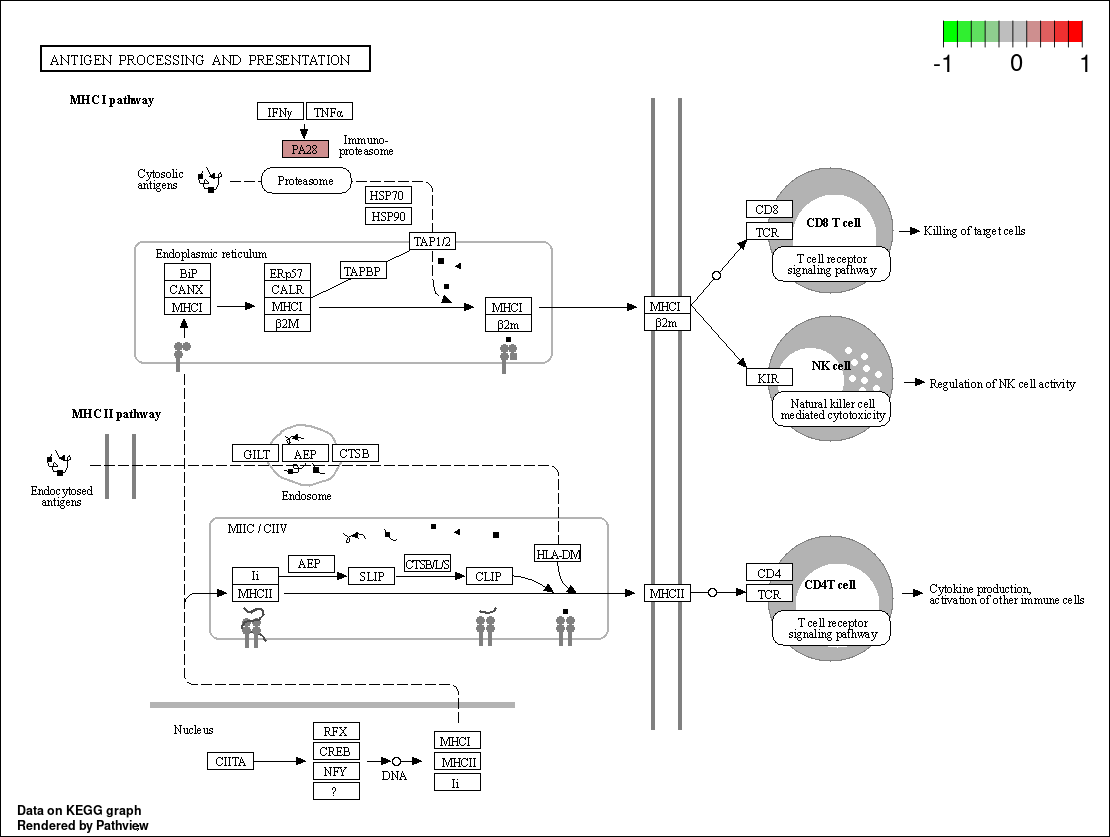
\includegraphics[width = 0.9\linewidth]{pathview2024-03-08_13_57_04.806626/hsa04612.pathview.png}
\caption{PPS PPI hsa04612 visualization}\label{fig:PPS-PPI-hsa04612-visualization}
\end{center}

\hypertarget{cut-ppi}{%
\subsubsection{根据富集结果缩减 PPI}\label{cut-ppi}}

由于富集结果可以凸显肿瘤的性质,这里尝试根据 KEGG top 10 通路的富集基因缩减 PPI

Figure \ref{fig:PPS-DPS-filtered-by-KEGG-and-formated-PPI-network} (下方图) 为图PPS DPS filtered by KEGG and formated PPI network概览。

\textbf{(对应文件为 \texttt{Figure+Table/PPS-DPS-filtered-by-KEGG-and-formated-PPI-network.pdf})}

\def\@captype{figure}
\begin{center}
\includegraphics[width = 0.9\linewidth]{Figure+Table/PPS-DPS-filtered-by-KEGG-and-formated-PPI-network.pdf}
\caption{PPS DPS filtered by KEGG and formated PPI network}\label{fig:PPS-DPS-filtered-by-KEGG-and-formated-PPI-network}
\end{center}

Figure \ref{fig:PPS-DPS-filtered-by-KEGG-Top-MCC-score} (下方图) 为图PPS DPS filtered by KEGG Top MCC score概览。

\textbf{(对应文件为 \texttt{Figure+Table/PPS-DPS-filtered-by-KEGG-Top-MCC-score.pdf})}

\def\@captype{figure}
\begin{center}
\includegraphics[width = 0.9\linewidth]{Figure+Table/PPS-DPS-filtered-by-KEGG-Top-MCC-score.pdf}
\caption{PPS DPS filtered by KEGG Top MCC score}\label{fig:PPS-DPS-filtered-by-KEGG-Top-MCC-score}
\end{center}

\hypertarget{workflow2}{%
\section{附:分析流程------耐药差异膜蛋白及对应抗体蛋白或互作抑制其表达蛋白}\label{workflow2}}

\hypertarget{ux7ed3ux80a0ux764cux5deeux5f02ux86cbux767d}{%
\subsection{结肠癌差异蛋白}\label{ux7ed3ux80a0ux764cux5deeux5f02ux86cbux767d}}

注:由于无法直接获得包含耐药性分组的蛋白表达数据,因此这部分的内容另寻思路,
即,获取 TCGA-COAD 的基因表达数据和蛋白定量数据,以 \texttt{pRRophetic} 根据基因表达数据
分析耐药性,再对样本分组,随后分析蛋白定量数据。

\hypertarget{ux6570ux636eux6765ux6e90-1}{%
\subsubsection{数据来源}\label{ux6570ux636eux6765ux6e90-1}}

共使用了 TCGA-COAD 的 RNA, protein, clinical 数据 (使用了三者都包含的病人的样本数据)。

Table \ref{tab:TCGA-COAD-clinical-metadata} (下方表格) 为表格TCGA COAD clinical metadata概览。

\textbf{(对应文件为 \texttt{Figure+Table/TCGA-COAD-clinical-metadata.csv})}

\begin{center}\begin{tcolorbox}[colback=gray!10, colframe=gray!50, width=0.9\linewidth, arc=1mm, boxrule=0.5pt]注:表格共有459行19列,以下预览的表格可能省略部分数据;表格含有459个唯一`rownames'。
\end{tcolorbox}
\end{center}

\begin{longtable}[]{@{}llllllllll@{}}
\caption{\label{tab:TCGA-COAD-clinical-metadata}TCGA COAD clinical metadata}\tabularnewline
\toprule
rownames & id & data\_f\ldots{} & cases & access & file\_name & submit\ldots{} & data\_c\ldots{} & type & file\_size\tabularnewline
\midrule
\endfirsthead
\toprule
rownames & id & data\_f\ldots{} & cases & access & file\_name & submit\ldots{} & data\_c\ldots{} & type & file\_size\tabularnewline
\midrule
\endhead
1 & 080f87\ldots{} & BCR XML & TCGA-A\ldots{} & open & nation\ldots{} & nation\ldots{} & Clinical & clinic\ldots{} & 29118\tabularnewline
2 & 77638e\ldots{} & BCR XML & TCGA-C\ldots{} & open & nation\ldots{} & nation\ldots{} & Clinical & clinic\ldots{} & 54636\tabularnewline
3 & c58a3b\ldots{} & BCR XML & TCGA-D\ldots{} & open & nation\ldots{} & nation\ldots{} & Clinical & clinic\ldots{} & 29261\tabularnewline
4 & e67964\ldots{} & BCR XML & TCGA-A\ldots{} & open & nation\ldots{} & nation\ldots{} & Clinical & clinic\ldots{} & 28673\tabularnewline
5 & 568223\ldots{} & BCR XML & TCGA-A\ldots{} & open & nation\ldots{} & nation\ldots{} & Clinical & clinic\ldots{} & 31577\tabularnewline
6 & d77499\ldots{} & BCR XML & TCGA-A\ldots{} & open & nation\ldots{} & nation\ldots{} & Clinical & clinic\ldots{} & 31559\tabularnewline
7 & 0efd65\ldots{} & BCR XML & TCGA-A\ldots{} & open & nation\ldots{} & nation\ldots{} & Clinical & clinic\ldots{} & 29185\tabularnewline
8 & 7aaa95\ldots{} & BCR XML & TCGA-A\ldots{} & open & nation\ldots{} & nation\ldots{} & Clinical & clinic\ldots{} & 52563\tabularnewline
9 & 75bb5e\ldots{} & BCR XML & TCGA-G\ldots{} & open & nation\ldots{} & nation\ldots{} & Clinical & clinic\ldots{} & 54330\tabularnewline
10 & 5d3d27\ldots{} & BCR XML & TCGA-D\ldots{} & open & nation\ldots{} & nation\ldots{} & Clinical & clinic\ldots{} & 29453\tabularnewline
11 & 0f0694\ldots{} & BCR XML & TCGA-A\ldots{} & open & nation\ldots{} & nation\ldots{} & Clinical & clinic\ldots{} & 24277\tabularnewline
12 & d05b7b\ldots{} & BCR XML & TCGA-A\ldots{} & open & nation\ldots{} & nation\ldots{} & Clinical & clinic\ldots{} & 34479\tabularnewline
13 & ef4172\ldots{} & BCR XML & TCGA-A\ldots{} & open & nation\ldots{} & nation\ldots{} & Clinical & clinic\ldots{} & 24264\tabularnewline
14 & f64700\ldots{} & BCR XML & TCGA-G\ldots{} & open & nation\ldots{} & nation\ldots{} & Clinical & clinic\ldots{} & 29321\tabularnewline
15 & 849b28\ldots{} & BCR XML & TCGA-A\ldots{} & open & nation\ldots{} & nation\ldots{} & Clinical & clinic\ldots{} & 24215\tabularnewline
\ldots{} & \ldots{} & \ldots{} & \ldots{} & \ldots{} & \ldots{} & \ldots{} & \ldots{} & \ldots{} & \ldots{}\tabularnewline
\bottomrule
\end{longtable}

Table \ref{tab:TCGA-COAD-protein-metadata} (下方表格) 为表格TCGA COAD protein metadata概览。

\textbf{(对应文件为 \texttt{Figure+Table/TCGA-COAD-protein-metadata.csv})}

\begin{center}\begin{tcolorbox}[colback=gray!10, colframe=gray!50, width=0.9\linewidth, arc=1mm, boxrule=0.5pt]注:表格共有363行24列,以下预览的表格可能省略部分数据;表格含有363个唯一`id'。
\end{tcolorbox}
\end{center}

\begin{longtable}[]{@{}llllllllll@{}}
\caption{\label{tab:TCGA-COAD-protein-metadata}TCGA COAD protein metadata}\tabularnewline
\toprule
id & data\_f\ldots{} & cases & access & file\_name & submit\ldots{} & data\_c\ldots{} & type & platform & file\_size\tabularnewline
\midrule
\endfirsthead
\toprule
id & data\_f\ldots{} & cases & access & file\_name & submit\ldots{} & data\_c\ldots{} & type & platform & file\_size\tabularnewline
\midrule
\endhead
7b5dc5\ldots{} & TSV & TCGA-C\ldots{} & open & TCGA-C\ldots{} & TCGA-C\ldots{} & Proteo\ldots{} & protei\ldots{} & RPPA & 22135\tabularnewline
7d66e7\ldots{} & TSV & TCGA-S\ldots{} & open & TCGA-S\ldots{} & TCGA-S\ldots{} & Proteo\ldots{} & protei\ldots{} & RPPA & 22022\tabularnewline
8ecf75\ldots{} & TSV & TCGA-A\ldots{} & open & TCGA-A\ldots{} & TCGA-A\ldots{} & Proteo\ldots{} & protei\ldots{} & RPPA & 24055\tabularnewline
5e4ec1\ldots{} & TSV & TCGA-A\ldots{} & open & TCGA-A\ldots{} & TCGA-A\ldots{} & Proteo\ldots{} & protei\ldots{} & RPPA & 23999\tabularnewline
e45a96\ldots{} & TSV & TCGA-A\ldots{} & open & TCGA-A\ldots{} & TCGA-A\ldots{} & Proteo\ldots{} & protei\ldots{} & RPPA & 24027\tabularnewline
47c932\ldots{} & TSV & TCGA-C\ldots{} & open & TCGA-C\ldots{} & TCGA-C\ldots{} & Proteo\ldots{} & protei\ldots{} & RPPA & 22100\tabularnewline
44f0f7\ldots{} & TSV & TCGA-A\ldots{} & open & TCGA-A\ldots{} & TCGA-A\ldots{} & Proteo\ldots{} & protei\ldots{} & RPPA & 24049\tabularnewline
9fe863\ldots{} & TSV & TCGA-C\ldots{} & open & TCGA-C\ldots{} & TCGA-C\ldots{} & Proteo\ldots{} & protei\ldots{} & RPPA & 22071\tabularnewline
e06fe7\ldots{} & TSV & TCGA-A\ldots{} & open & TCGA-A\ldots{} & TCGA-A\ldots{} & Proteo\ldots{} & protei\ldots{} & RPPA & 24065\tabularnewline
cf9c71\ldots{} & TSV & TCGA-Q\ldots{} & open & TCGA-Q\ldots{} & TCGA-Q\ldots{} & Proteo\ldots{} & protei\ldots{} & RPPA & 22099\tabularnewline
335dae\ldots{} & TSV & TCGA-G\ldots{} & open & TCGA-G\ldots{} & TCGA-G\ldots{} & Proteo\ldots{} & protei\ldots{} & RPPA & 22154\tabularnewline
4f0d60\ldots{} & TSV & TCGA-D\ldots{} & open & TCGA-D\ldots{} & TCGA-D\ldots{} & Proteo\ldots{} & protei\ldots{} & RPPA & 22155\tabularnewline
f36bba\ldots{} & TSV & TCGA-G\ldots{} & open & TCGA-G\ldots{} & TCGA-G\ldots{} & Proteo\ldots{} & protei\ldots{} & RPPA & 22109\tabularnewline
f185df\ldots{} & TSV & TCGA-A\ldots{} & open & TCGA-A\ldots{} & TCGA-A\ldots{} & Proteo\ldots{} & protei\ldots{} & RPPA & 24011\tabularnewline
be6d80\ldots{} & TSV & TCGA-F\ldots{} & open & TCGA-F\ldots{} & TCGA-F\ldots{} & Proteo\ldots{} & protei\ldots{} & RPPA & 22109\tabularnewline
\ldots{} & \ldots{} & \ldots{} & \ldots{} & \ldots{} & \ldots{} & \ldots{} & \ldots{} & \ldots{} & \ldots{}\tabularnewline
\bottomrule
\end{longtable}

Table \ref{tab:TCGA-COAD-RNA-metadata} (下方表格) 为表格TCGA COAD RNA metadata概览。

\textbf{(对应文件为 \texttt{Figure+Table/TCGA-COAD-RNA-metadata.csv})}

\begin{center}\begin{tcolorbox}[colback=gray!10, colframe=gray!50, width=0.9\linewidth, arc=1mm, boxrule=0.5pt]注:表格共有524行29列,以下预览的表格可能省略部分数据;表格含有524个唯一`id'。
\end{tcolorbox}
\end{center}

\begin{longtable}[]{@{}llllllllll@{}}
\caption{\label{tab:TCGA-COAD-RNA-metadata}TCGA COAD RNA metadata}\tabularnewline
\toprule
id & data\_f\ldots{} & cases & access & file\_name & submit\ldots{} & data\_c\ldots{} & type & file\_size & create\ldots{}\tabularnewline
\midrule
\endfirsthead
\toprule
id & data\_f\ldots{} & cases & access & file\_name & submit\ldots{} & data\_c\ldots{} & type & file\_size & create\ldots{}\tabularnewline
\midrule
\endhead
efdcda\ldots{} & TSV & TCGA-C\ldots{} & open & a45a75\ldots{} & 9a7d8c\ldots{} & Transc\ldots{} & gene\_e\ldots{} & 4240354 & 2022-0\ldots{}\tabularnewline
66905c\ldots{} & TSV & TCGA-A\ldots{} & open & 40b98f\ldots{} & 7070f7\ldots{} & Transc\ldots{} & gene\_e\ldots{} & 4233852 & 2022-0\ldots{}\tabularnewline
8820d9\ldots{} & TSV & TCGA-A\ldots{} & open & 58369b\ldots{} & a6da34\ldots{} & Transc\ldots{} & gene\_e\ldots{} & 4210387 & 2022-0\ldots{}\tabularnewline
5302ca\ldots{} & TSV & TCGA-C\ldots{} & open & 45a267\ldots{} & c5db3d\ldots{} & Transc\ldots{} & gene\_e\ldots{} & 4209007 & 2022-0\ldots{}\tabularnewline
a7affc\ldots{} & TSV & TCGA-A\ldots{} & open & 3ef878\ldots{} & 97c2f0\ldots{} & Transc\ldots{} & gene\_e\ldots{} & 4208716 & 2022-0\ldots{}\tabularnewline
3456d4\ldots{} & TSV & TCGA-A\ldots{} & open & 524723\ldots{} & 4d8cb5\ldots{} & Transc\ldots{} & gene\_e\ldots{} & 4216110 & 2022-0\ldots{}\tabularnewline
ab6d59\ldots{} & TSV & TCGA-G\ldots{} & open & 085e42\ldots{} & 228266\ldots{} & Transc\ldots{} & gene\_e\ldots{} & 4231843 & 2022-0\ldots{}\tabularnewline
3db2cc\ldots{} & TSV & TCGA-A\ldots{} & open & e1d0ac\ldots{} & 2b637e\ldots{} & Transc\ldots{} & gene\_e\ldots{} & 4210406 & 2022-0\ldots{}\tabularnewline
a761bd\ldots{} & TSV & TCGA-A\ldots{} & open & d837c3\ldots{} & 738864\ldots{} & Transc\ldots{} & gene\_e\ldots{} & 4201059 & 2022-0\ldots{}\tabularnewline
04981c\ldots{} & TSV & TCGA-A\ldots{} & open & 4bafe8\ldots{} & 53e5cd\ldots{} & Transc\ldots{} & gene\_e\ldots{} & 4214788 & 2022-0\ldots{}\tabularnewline
8ac00c\ldots{} & TSV & TCGA-A\ldots{} & open & 0ae6d3\ldots{} & 0e343a\ldots{} & Transc\ldots{} & gene\_e\ldots{} & 4219902 & 2022-0\ldots{}\tabularnewline
e929b2\ldots{} & TSV & TCGA-C\ldots{} & open & a82c20\ldots{} & 99e86d\ldots{} & Transc\ldots{} & gene\_e\ldots{} & 4223537 & 2022-0\ldots{}\tabularnewline
c403bb\ldots{} & TSV & TCGA-A\ldots{} & open & e5ae4a\ldots{} & 8e4b41\ldots{} & Transc\ldots{} & gene\_e\ldots{} & 4211960 & 2022-0\ldots{}\tabularnewline
756b10\ldots{} & TSV & TCGA-A\ldots{} & open & b3e428\ldots{} & fe34e7\ldots{} & Transc\ldots{} & gene\_e\ldots{} & 4229447 & 2022-0\ldots{}\tabularnewline
700b39\ldots{} & TSV & TCGA-A\ldots{} & open & fd618c\ldots{} & afa933\ldots{} & Transc\ldots{} & gene\_e\ldots{} & 4229363 & 2022-0\ldots{}\tabularnewline
\ldots{} & \ldots{} & \ldots{} & \ldots{} & \ldots{} & \ldots{} & \ldots{} & \ldots{} & \ldots{} & \ldots{}\tabularnewline
\bottomrule
\end{longtable}

\hypertarget{ux9884ux6d4bux8010ux836fux6027}{%
\subsection{预测耐药性}\label{ux9884ux6d4bux8010ux836fux6027}}

\hypertarget{ux4f7fux7528-rna-ux6570ux636eux96c6ux9884ux6d4b}{%
\subsubsection{使用 RNA 数据集预测}\label{ux4f7fux7528-rna-ux6570ux636eux96c6ux9884ux6d4b}}

以 \texttt{pRRophetic} 预测药物敏感性 (Cisplatin)。

Figure \ref{fig:QQ-plot-for-distribution-of-the-transformed-IC50-data} (下方图) 为图QQ plot for distribution of the transformed IC50 data概览。

\textbf{(对应文件为 \texttt{Figure+Table/QQ-plot-for-distribution-of-the-transformed-IC50-data.pdf})}

\def\@captype{figure}
\begin{center}
\includegraphics[width = 0.9\linewidth]{Figure+Table/QQ-plot-for-distribution-of-the-transformed-IC50-data.pdf}
\caption{QQ plot for distribution of the transformed IC50 data}\label{fig:QQ-plot-for-distribution-of-the-transformed-IC50-data}
\end{center}

Fig. \ref{fig:QQ-plot-for-distribution-of-the-transformed-IC50-data} 表明,
Cisplatin 的 IC\textsubscript{50} 数据特征基本符合正太分布,可以用于线形预测 Cisplatin 敏感性。

Figure \ref{fig:Estimate-prediction-accuracy} (下方图) 为图Estimate prediction accuracy概览。

\textbf{(对应文件为 \texttt{Figure+Table/Estimate-prediction-accuracy.pdf})}

\def\@captype{figure}
\begin{center}
\includegraphics[width = 0.9\linewidth]{Figure+Table/Estimate-prediction-accuracy.pdf}
\caption{Estimate prediction accuracy}\label{fig:Estimate-prediction-accuracy}
\end{center}

\begin{center}\begin{tcolorbox}[colback=gray!10, colframe=gray!50, width=0.9\linewidth, arc=1mm, boxrule=0.5pt]
\textbf{
k-means clustering
:}

\vspace{0.5em}

    Centers = 3

\vspace{2em}
\end{tcolorbox}
\end{center}

Table \ref{tab:Predicted-drug-sensitivity} (下方表格) 为表格Predicted drug sensitivity概览。

\textbf{(对应文件为 \texttt{Figure+Table/Predicted-drug-sensitivity.csv})}

\begin{center}\begin{tcolorbox}[colback=gray!10, colframe=gray!50, width=0.9\linewidth, arc=1mm, boxrule=0.5pt]注:表格共有357行3列,以下预览的表格可能省略部分数据;表格含有357个唯一`sample'。
\end{tcolorbox}
\end{center}
\begin{center}\begin{tcolorbox}[colback=gray!10, colframe=gray!50, width=0.9\linewidth, arc=1mm, boxrule=0.5pt]\begin{enumerate}\tightlist
\item sample:  样品名称
\end{enumerate}\end{tcolorbox}
\end{center}

\begin{longtable}[]{@{}lll@{}}
\caption{\label{tab:Predicted-drug-sensitivity}Predicted drug sensitivity}\tabularnewline
\toprule
sample & sensitivity & kmeans\_group\tabularnewline
\midrule
\endfirsthead
\toprule
sample & sensitivity & kmeans\_group\tabularnewline
\midrule
\endhead
TCGA-3L-AA1B-01A & 4.14816093273104 & 2\tabularnewline
TCGA-4N-A93T-01A & 4.40190686256072 & 2\tabularnewline
TCGA-4T-AA8H-01A & 4.15648471482818 & 2\tabularnewline
TCGA-5M-AAT6-01A & 2.62116649131769 & 3\tabularnewline
TCGA-A6-2671-11A & 4.03864919730421 & 2\tabularnewline
TCGA-A6-2672-01A & 2.76158089020952 & 3\tabularnewline
TCGA-A6-2676-01A & 2.10216420226229 & 3\tabularnewline
TCGA-A6-2677-01A & 3.02480062454453 & 1\tabularnewline
TCGA-A6-2678-11A & 3.85525962252971 & 2\tabularnewline
TCGA-A6-2680-01A & 4.07942930425798 & 2\tabularnewline
TCGA-A6-2681-01A & 3.95239422637806 & 2\tabularnewline
TCGA-A6-2683-11A & 3.64057626378351 & 1\tabularnewline
TCGA-A6-2684-01C & 2.93670056076102 & 3\tabularnewline
TCGA-A6-2685-01A & 4.32047341962156 & 2\tabularnewline
TCGA-A6-2686-11A & 3.87165483393886 & 2\tabularnewline
\ldots{} & \ldots{} & \ldots{}\tabularnewline
\bottomrule
\end{longtable}

\hypertarget{ux5deeux5f02ux86cbux767dux7b5bux9009}{%
\subsection{差异蛋白筛选}\label{ux5deeux5f02ux86cbux767dux7b5bux9009}}

\hypertarget{ux5143ux6570ux636e}{%
\subsubsection{元数据}\label{ux5143ux6570ux636e}}

根据 Tab. \ref{tab:Predicted-drug-sensitivity} k-means 聚类结果,将
样品分为三组:耐药组、中等组、低耐药性组 (非耐药组) 。

\begin{center}\begin{tcolorbox}[colback=gray!10, colframe=gray!50, width=0.9\linewidth, arc=1mm, boxrule=0.5pt]
\textbf{
k-means clustering
:}

\vspace{0.5em}

    Centers = 3

\vspace{2em}
\end{tcolorbox}
\end{center}

Table \ref{tab:TCGA-COAD-proteome-metadata} (下方表格) 为表格TCGA COAD proteome metadata概览。

\textbf{(对应文件为 \texttt{Figure+Table/TCGA-COAD-proteome-metadata.csv})}

\begin{center}\begin{tcolorbox}[colback=gray!10, colframe=gray!50, width=0.9\linewidth, arc=1mm, boxrule=0.5pt]注:表格共有178行4列,以下预览的表格可能省略部分数据;表格含有2个唯一`group'。
\end{tcolorbox}
\end{center}
\begin{center}\begin{tcolorbox}[colback=gray!10, colframe=gray!50, width=0.9\linewidth, arc=1mm, boxrule=0.5pt]\begin{enumerate}\tightlist
\item sample:  样品名称
\item group:  分组名称
\end{enumerate}\end{tcolorbox}
\end{center}

\begin{longtable}[]{@{}llll@{}}
\caption{\label{tab:TCGA-COAD-proteome-metadata}TCGA COAD proteome metadata}\tabularnewline
\toprule
sample & group & sensitivity & kmeans\_group\tabularnewline
\midrule
\endfirsthead
\toprule
sample & group & sensitivity & kmeans\_group\tabularnewline
\midrule
\endhead
TCGA-3L-AA1B & Resistance & 4.14816093273104 & 2\tabularnewline
TCGA-4N-A93T & Resistance & 4.40190686256072 & 2\tabularnewline
TCGA-4T-AA8H & Resistance & 4.15648471482818 & 2\tabularnewline
TCGA-5M-AAT6 & Non\_resistance & 2.62116649131769 & 3\tabularnewline
TCGA-A6-2671 & Resistance & 4.03864919730421 & 2\tabularnewline
TCGA-A6-2672 & Non\_resistance & 2.76158089020952 & 3\tabularnewline
TCGA-A6-2676 & Non\_resistance & 2.10216420226229 & 3\tabularnewline
TCGA-A6-2678 & Resistance & 3.85525962252971 & 2\tabularnewline
TCGA-A6-2680 & Resistance & 4.07942930425798 & 2\tabularnewline
TCGA-A6-2681 & Resistance & 3.95239422637806 & 2\tabularnewline
TCGA-A6-2684 & Non\_resistance & 2.93670056076102 & 3\tabularnewline
TCGA-A6-2685 & Resistance & 4.32047341962156 & 2\tabularnewline
TCGA-A6-2686 & Resistance & 3.87165483393886 & 2\tabularnewline
TCGA-A6-3808 & Non\_resistance & 2.93134891159939 & 3\tabularnewline
TCGA-A6-3809 & Non\_resistance & 1.43580359549368 & 3\tabularnewline
\ldots{} & \ldots{} & \ldots{} & \ldots{}\tabularnewline
\bottomrule
\end{longtable}

\hypertarget{ux5deeux5f02ux86cbux767d-1}{%
\subsubsection{差异蛋白}\label{ux5deeux5f02ux86cbux767d-1}}

Figure \ref{fig:TCGA-Resistance-vs-Non-resistance-DEPs} (下方图) 为图TCGA Resistance vs Non resistance DEPs概览。

\textbf{(对应文件为 \texttt{Figure+Table/TCGA-Resistance-vs-Non-resistance-DEPs.pdf})}

\def\@captype{figure}
\begin{center}
\includegraphics[width = 0.9\linewidth]{Figure+Table/TCGA-Resistance-vs-Non-resistance-DEPs.pdf}
\caption{TCGA Resistance vs Non resistance DEPs}\label{fig:TCGA-Resistance-vs-Non-resistance-DEPs}
\end{center}

Table \ref{tab:TCGA-data-Resistance-vs-Non-resistance-DEPs} (下方表格) 为表格TCGA data Resistance vs Non resistance DEPs概览。

\textbf{(对应文件为 \texttt{Figure+Table/TCGA-data-Resistance-vs-Non-resistance-DEPs.csv})}

\begin{center}\begin{tcolorbox}[colback=gray!10, colframe=gray!50, width=0.9\linewidth, arc=1mm, boxrule=0.5pt]注:表格共有30行9列,以下预览的表格可能省略部分数据;表格含有30个唯一`rownames'。
\end{tcolorbox}
\end{center}
\begin{center}\begin{tcolorbox}[colback=gray!10, colframe=gray!50, width=0.9\linewidth, arc=1mm, boxrule=0.5pt]\begin{enumerate}\tightlist
\item logFC:  estimate of the log2-fold-change corresponding to the effect or contrast (for ‘topTableF’ there may be several columns of log-fold-changes)
\item AveExpr:  average log2-expression for the probe over all arrays and channels, same as ‘Amean’ in the ‘MarrayLM’ object
\item t:  moderated t-statistic (omitted for ‘topTableF’)
\item P.Value:  raw p-value
\item B:  log-odds that the gene is differentially expressed (omitted for ‘topTreat’)
\end{enumerate}\end{tcolorbox}
\end{center}

\begin{longtable}[]{@{}lllllllll@{}}
\caption{\label{tab:TCGA-data-Resistance-vs-Non-resistance-DEPs}TCGA data Resistance vs Non resistance DEPs}\tabularnewline
\toprule
rownames & logFC & AveExpr & t & P.Value & adj.P.Val & B & peptid\ldots{} & Gene\_name\tabularnewline
\midrule
\endfirsthead
\toprule
rownames & logFC & AveExpr & t & P.Value & adj.P.Val & B & peptid\ldots{} & Gene\_name\tabularnewline
\midrule
\endhead
AGID00319 & -0.598\ldots{} & 0.0565\ldots{} & -7.018\ldots{} & 4.6950\ldots{} & 2.1691\ldots{} & 14.789\ldots{} & Granzy\ldots{} & Granzy\ldots{}\tabularnewline
AGID00015 & -0.903\ldots{} & 0.7403\ldots{} & -5.932\ldots{} & 1.5134\ldots{} & 2.3504\ldots{} & 9.2486\ldots{} & CASPAS\ldots{} & CASPAS\ldots{}\tabularnewline
AGID00155 & 0.3382\ldots{} & 0.2485\ldots{} & 5.9309\ldots{} & 1.5262\ldots{} & 2.3504\ldots{} & 9.2406\ldots{} & TSC1 & TSC1\tabularnewline
AGID00366 & -0.845\ldots{} & 1.0622\ldots{} & -5.114\ldots{} & 8.1696\ldots{} & 5.3919\ldots{} & 5.4545\ldots{} & IDO & IDO\tabularnewline
AGID00193 & -0.371\ldots{} & -0.473\ldots{} & -4.922\ldots{} & 1.9302\ldots{} & 0.0001\ldots{} & 4.6336\ldots{} & ANNEXIN1 & ANNEXIN1\tabularnewline
AGID00268 & 0.4910\ldots{} & -0.646\ldots{} & 4.7228\ldots{} & 4.7425\ldots{} & 0.0002\ldots{} & 3.7904\ldots{} & ATRX & ATRX\tabularnewline
AGID02153 & 0.3689\ldots{} & 0.4742\ldots{} & 4.6151\ldots{} & 7.4803\ldots{} & 0.0003\ldots{} & 3.3539\ldots{} & INPP4B & INPP4B\tabularnewline
AGID00053 & -0.486\ldots{} & 0.1941\ldots{} & -4.609\ldots{} & 7.6492\ldots{} & 0.0003\ldots{} & 3.3328\ldots{} & PAI1 & PAI1\tabularnewline
AGID00450 & 0.4087\ldots{} & 0.5620\ldots{} & 4.5837\ldots{} & 8.5582\ldots{} & 0.0003\ldots{} & 3.2270\ldots{} & EGFR\_p\ldots{} & EGFR\_p\ldots{}\tabularnewline
AGID00235 & -1.143\ldots{} & -0.300\ldots{} & -4.562\ldots{} & 9.4475\ldots{} & 0.0003\ldots{} & 3.1408\ldots{} & EMA & EMA\tabularnewline
AGID00394 & -0.365\ldots{} & 0.1766\ldots{} & -4.503\ldots{} & 1.2172\ldots{} & 0.0003\ldots{} & 2.9023\ldots{} & Enolase-1 & Enolase-1\tabularnewline
AGID00031 & -0.384\ldots{} & -0.126\ldots{} & -4.410\ldots{} & 1.7819\ldots{} & 0.0004\ldots{} & 2.5371\ldots{} & FIBRON\ldots{} & FIBRON\ldots{}\tabularnewline
AGID00290 & 0.3109\ldots{} & -0.549\ldots{} & 4.3319\ldots{} & 2.4809\ldots{} & 0.0006\ldots{} & 2.2336\ldots{} & Lasu1 & Lasu1\tabularnewline
AGID00148 & 0.6118\ldots{} & 0.3484\ldots{} & 4.3171\ldots{} & 2.6150\ldots{} & 0.0006\ldots{} & 2.1771\ldots{} & ECADHERIN & ECADHERIN\tabularnewline
AGID00301 & -0.312\ldots{} & -0.132\ldots{} & -4.125\ldots{} & 5.6927\ldots{} & 0.0011\ldots{} & 1.4564\ldots{} & B7-H3 & B7-H3\tabularnewline
\ldots{} & \ldots{} & \ldots{} & \ldots{} & \ldots{} & \ldots{} & \ldots{} & \ldots{} & \ldots{}\tabularnewline
\bottomrule
\end{longtable}

\hypertarget{ux819cux86cbux767dux7b5bux9009-1}{%
\subsection{膜蛋白筛选}\label{ux819cux86cbux767dux7b5bux9009-1}}

\hypertarget{unitmp-1}{%
\subsubsection{Unitmp}\label{unitmp-1}}

UniTmp: unified resources for transmembrane proteins\textsuperscript{\protect\hyperlink{ref-UnitmpUnifiedDobson2024}{9}}

见 Tab. \ref{tab:UniTmp-data-of-htp-all}

\hypertarget{ux4e0eux9ad8ux8868ux8fbeux5deeux5f02ux86cbux767d-tcga-dps-up-ux4ea4ux96c6}{%
\subsubsection{与高表达差异蛋白 (TCGA-dps-Up) 交集}\label{ux4e0eux9ad8ux8868ux8fbeux5deeux5f02ux86cbux767d-tcga-dps-up-ux4ea4ux96c6}}

Figure \ref{fig:TCGA-Intersection-of-DPs-Up-with-TransMemPs} (下方图) 为图TCGA Intersection of DPs Up with TransMemPs概览。

\textbf{(对应文件为 \texttt{Figure+Table/TCGA-Intersection-of-DPs-Up-with-TransMemPs.pdf})}

\def\@captype{figure}
\begin{center}
\includegraphics[width = 0.9\linewidth]{Figure+Table/TCGA-Intersection-of-DPs-Up-with-TransMemPs.pdf}
\caption{TCGA Intersection of DPs Up with TransMemPs}\label{fig:TCGA-Intersection-of-DPs-Up-with-TransMemPs}
\end{center}
\begin{center}\begin{tcolorbox}[colback=gray!10, colframe=gray!50, width=0.9\linewidth, arc=1mm, boxrule=0.5pt]
\textbf{
Intersection
:}

\vspace{0.5em}

    TSC1

\vspace{2em}
\end{tcolorbox}
\end{center}

\textbf{(上述信息框内容已保存至 \texttt{Figure+Table/TCGA-Intersection-of-DPs-Up-with-TransMemPs-content})}

\hypertarget{ux4ee5ux86cbux767dux4e92ux4f5cux7b5bux9009ux914dux4f53ux86cbux767d-1}{%
\subsection{以蛋白互作筛选配体蛋白}\label{ux4ee5ux86cbux767dux4e92ux4f5cux7b5bux9009ux914dux4f53ux86cbux767d-1}}

\hypertarget{tcga-coad-ux7684-rna-seq-ux5deeux5f02ux8868ux8fbe}{%
\subsubsection{TCGA-COAD 的 RNA-seq 差异表达}\label{tcga-coad-ux7684-rna-seq-ux5deeux5f02ux8868ux8fbe}}

为了筛选 Fig. \ref{fig:TCGA-Intersection-of-DPs-Up-with-TransMemPs} 的配体,
以 TCGA-COAD 的差异表达基因作为候选。

Figure \ref{fig:TCGA-RNA-Resistance-vs-Non-resistance-DEGs} (下方图) 为图TCGA RNA Resistance vs Non resistance DEGs概览。

\textbf{(对应文件为 \texttt{Figure+Table/TCGA-RNA-Resistance-vs-Non-resistance-DEGs.pdf})}

\def\@captype{figure}
\begin{center}
\includegraphics[width = 0.9\linewidth]{Figure+Table/TCGA-RNA-Resistance-vs-Non-resistance-DEGs.pdf}
\caption{TCGA RNA Resistance vs Non resistance DEGs}\label{fig:TCGA-RNA-Resistance-vs-Non-resistance-DEGs}
\end{center}

Table \ref{tab:TCGA-RNA-data-Resistance-vs-Non-resistance-DEGs} (下方表格) 为表格TCGA RNA data Resistance vs Non resistance DEGs概览。

\textbf{(对应文件为 \texttt{Figure+Table/TCGA-RNA-data-Resistance-vs-Non-resistance-DEGs.csv})}

\begin{center}\begin{tcolorbox}[colback=gray!10, colframe=gray!50, width=0.9\linewidth, arc=1mm, boxrule=0.5pt]注:表格共有10108行22列,以下预览的表格可能省略部分数据;表格含有10108个唯一`rownames'。
\end{tcolorbox}
\end{center}
\begin{center}\begin{tcolorbox}[colback=gray!10, colframe=gray!50, width=0.9\linewidth, arc=1mm, boxrule=0.5pt]\begin{enumerate}\tightlist
\item logFC:  estimate of the log2-fold-change corresponding to the effect or contrast (for ‘topTableF’ there may be several columns of log-fold-changes)
\item AveExpr:  average log2-expression for the probe over all arrays and channels, same as ‘Amean’ in the ‘MarrayLM’ object
\item t:  moderated t-statistic (omitted for ‘topTableF’)
\item P.Value:  raw p-value
\item B:  log-odds that the gene is differentially expressed (omitted for ‘topTreat’)
\item gene\_id:  GENCODE/Ensembl gene ID
\item gene\_name:  GENCODE gene name
\item strand:  genomic strand
\end{enumerate}\end{tcolorbox}
\end{center}

\begin{longtable}[]{@{}llllllllll@{}}
\caption{\label{tab:TCGA-RNA-data-Resistance-vs-Non-resistance-DEGs}TCGA RNA data Resistance vs Non resistance DEGs}\tabularnewline
\toprule
rownames & gene\_id & seqnames & start & end & width & strand & source & type & score\tabularnewline
\midrule
\endfirsthead
\toprule
rownames & gene\_id & seqnames & start & end & width & strand & source & type & score\tabularnewline
\midrule
\endhead
ENSG00\ldots{} & ENSG00\ldots{} & chr5 & 132822141 & 132830659 & 8519 & - & HAVANA & gene & NA\tabularnewline
ENSG00\ldots{} & ENSG00\ldots{} & chr16 & 89818179 & 89871319 & 53141 & + & HAVANA & gene & NA\tabularnewline
ENSG00\ldots{} & ENSG00\ldots{} & chr12 & 98613405 & 98645113 & 31709 & - & HAVANA & gene & NA\tabularnewline
ENSG00\ldots{} & ENSG00\ldots{} & chr16 & 3027682 & 3036944 & 9263 & - & HAVANA & gene & NA\tabularnewline
ENSG00\ldots{} & ENSG00\ldots{} & chr7 & 1542235 & 1560821 & 18587 & - & HAVANA & gene & NA\tabularnewline
ENSG00\ldots{} & ENSG00\ldots{} & chr9 & 128108581 & 128118693 & 10113 & - & HAVANA & gene & NA\tabularnewline
ENSG00\ldots{} & ENSG00\ldots{} & chr20 & 32443059 & 32585074 & 142016 & - & HAVANA & gene & NA\tabularnewline
ENSG00\ldots{} & ENSG00\ldots{} & chr11 & 417933 & 442011 & 24079 & - & HAVANA & gene & NA\tabularnewline
ENSG00\ldots{} & ENSG00\ldots{} & chr14 & 67360328 & 67386516 & 26189 & + & HAVANA & gene & NA\tabularnewline
ENSG00\ldots{} & ENSG00\ldots{} & chr7 & 101195007 & 101201038 & 6032 & - & HAVANA & gene & NA\tabularnewline
ENSG00\ldots{} & ENSG00\ldots{} & chr12 & 56230049 & 56237846 & 7798 & + & HAVANA & gene & NA\tabularnewline
ENSG00\ldots{} & ENSG00\ldots{} & chr3 & 48403854 & 48430086 & 26233 & - & HAVANA & gene & NA\tabularnewline
ENSG00\ldots{} & ENSG00\ldots{} & chr3 & 42489299 & 42537573 & 48275 & + & HAVANA & gene & NA\tabularnewline
ENSG00\ldots{} & ENSG00\ldots{} & chr17 & 79074824 & 79088599 & 13776 & + & HAVANA & gene & NA\tabularnewline
ENSG00\ldots{} & ENSG00\ldots{} & chr2 & 219054424 & 219060921 & 6498 & - & HAVANA & gene & NA\tabularnewline
\ldots{} & \ldots{} & \ldots{} & \ldots{} & \ldots{} & \ldots{} & \ldots{} & \ldots{} & \ldots{} & \ldots{}\tabularnewline
\bottomrule
\end{longtable}

Figure \ref{fig:TCGA-RNA-DEGs-type} (下方图) 为图TCGA RNA DEGs type概览。

\textbf{(对应文件为 \texttt{Figure+Table/TCGA-RNA-DEGs-type.pdf})}

\def\@captype{figure}
\begin{center}
\includegraphics[width = 0.9\linewidth]{Figure+Table/TCGA-RNA-DEGs-type.pdf}
\caption{TCGA RNA DEGs type}\label{fig:TCGA-RNA-DEGs-type}
\end{center}

\hypertarget{ppi-1}{%
\subsubsection{PPI}\label{ppi-1}}

以 Fig. \ref{fig:TCGA-Intersection-of-DPs-Up-with-TransMemPs} 和 Tab. \ref{tab:TCGA-RNA-data-Resistance-vs-Non-resistance-DEGs} top 2000 构建 PPI 网络。

Figure \ref{fig:TCGA-raw-PPI-network} (下方图) 为图TCGA raw PPI network概览。

\textbf{(对应文件为 \texttt{Figure+Table/TCGA-raw-PPI-network.pdf})}

\def\@captype{figure}
\begin{center}
\includegraphics[width = 0.9\linewidth]{Figure+Table/TCGA-raw-PPI-network.pdf}
\caption{TCGA raw PPI network}\label{fig:TCGA-raw-PPI-network}
\end{center}

将 PPI 网络过滤,凸显 Fig. \ref{fig:TCGA-Intersection-of-DPs-Up-with-TransMemPs} 交集蛋白 (MCC 筛选高分相连的其他蛋白)

Figure \ref{fig:TCGA-DPS-filtered-and-formated-PPI-network-logFC} (下方图) 为图TCGA DPS filtered and formated PPI network logFC概览。

\textbf{(对应文件为 \texttt{Figure+Table/TCGA-DPS-filtered-and-formated-PPI-network-logFC.pdf})}

\def\@captype{figure}
\begin{center}
\includegraphics[width = 0.9\linewidth]{Figure+Table/TCGA-DPS-filtered-and-formated-PPI-network-logFC.pdf}
\caption{TCGA DPS filtered and formated PPI network logFC}\label{fig:TCGA-DPS-filtered-and-formated-PPI-network-logFC}
\end{center}

Figure \ref{fig:TCGA-DPS-filtered-and-formated-PPI-network-MCC} (下方图) 为图TCGA DPS filtered and formated PPI network MCC概览。

\textbf{(对应文件为 \texttt{Figure+Table/TCGA-DPS-filtered-and-formated-PPI-network-MCC.pdf})}

\def\@captype{figure}
\begin{center}
\includegraphics[width = 0.9\linewidth]{Figure+Table/TCGA-DPS-filtered-and-formated-PPI-network-MCC.pdf}
\caption{TCGA DPS filtered and formated PPI network MCC}\label{fig:TCGA-DPS-filtered-and-formated-PPI-network-MCC}
\end{center}

\hypertarget{ux5bccux96c6ux5206ux6790-1}{%
\subsubsection{富集分析}\label{ux5bccux96c6ux5206ux6790-1}}

TSC1 在通路可见 Fig. \ref{fig:TCGA-TSC1-in-hsa04151-visualization}

Figure \ref{fig:TCGA-KEGG-enrichment} (下方图) 为图TCGA KEGG enrichment概览。

\textbf{(对应文件为 \texttt{Figure+Table/TCGA-KEGG-enrichment.pdf})}

\def\@captype{figure}
\begin{center}
\includegraphics[width = 0.9\linewidth]{Figure+Table/TCGA-KEGG-enrichment.pdf}
\caption{TCGA KEGG enrichment}\label{fig:TCGA-KEGG-enrichment}
\end{center}

Figure \ref{fig:TCGA-GO-enrichment} (下方图) 为图TCGA GO enrichment概览。

\textbf{(对应文件为 \texttt{Figure+Table/TCGA-GO-enrichment.pdf})}

\def\@captype{figure}
\begin{center}
\includegraphics[width = 0.9\linewidth]{Figure+Table/TCGA-GO-enrichment.pdf}
\caption{TCGA GO enrichment}\label{fig:TCGA-GO-enrichment}
\end{center}

Figure \ref{fig:TCGA-TSC1-in-hsa04151-visualization} (下方图) 为图TCGA TSC1 in hsa04151 visualization概览。

\textbf{(对应文件为 \texttt{Figure+Table/hsa04151.pathview.png})}

\def\@captype{figure}
\begin{center}
\includegraphics[width = 0.9\linewidth]{pathview2024-03-08_15_28_11.801928/hsa04151.pathview.png}
\caption{TCGA TSC1 in hsa04151 visualization}\label{fig:TCGA-TSC1-in-hsa04151-visualization}
\end{center}

\hypertarget{ux901aux8fc7ux5173ux8054ux5206ux6790ux7b5bux9009ux8d1fux76f8ux5173ux6027ux4e92ux4f5cux86cbux767d}{%
\subsubsection{通过关联分析筛选负相关性互作蛋白}\label{ux901aux8fc7ux5173ux8054ux5206ux6790ux7b5bux9009ux8d1fux76f8ux5173ux6027ux4e92ux4f5cux86cbux767d}}

Figure \ref{fig:TCGA-RNA-correlation-heatmap} (下方图) 为图TCGA RNA correlation heatmap概览。

\textbf{(对应文件为 \texttt{Figure+Table/TCGA-RNA-correlation-heatmap.pdf})}

\def\@captype{figure}
\begin{center}
\includegraphics[width = 0.9\linewidth]{Figure+Table/TCGA-RNA-correlation-heatmap.pdf}
\caption{TCGA RNA correlation heatmap}\label{fig:TCGA-RNA-correlation-heatmap}
\end{center}

Table \ref{tab:TCGA-RNA-TSC1-negtive-correlated} (下方表格) 为表格TCGA RNA TSC1 negtive correlated概览。

\textbf{(对应文件为 \texttt{Figure+Table/TCGA-RNA-TSC1-negtive-correlated.csv})}

\begin{center}\begin{tcolorbox}[colback=gray!10, colframe=gray!50, width=0.9\linewidth, arc=1mm, boxrule=0.5pt]注:表格共有5行7列,以下预览的表格可能省略部分数据;表格含有5个唯一`From'。
\end{tcolorbox}
\end{center}
\begin{center}\begin{tcolorbox}[colback=gray!10, colframe=gray!50, width=0.9\linewidth, arc=1mm, boxrule=0.5pt]\begin{enumerate}\tightlist
\item cor:  皮尔逊关联系数,正关联或负关联。
\item pvalue:  显著性 P。
\item -log2(P.value):  P 的对数转化。
\item significant:  显著性。
\item sign:  人为赋予的符号,参考 significant。
\end{enumerate}\end{tcolorbox}
\end{center}

\begin{longtable}[]{@{}lllllll@{}}
\caption{\label{tab:TCGA-RNA-TSC1-negtive-correlated}TCGA RNA TSC1 negtive correlated}\tabularnewline
\toprule
From & To & cor & pvalue & -log2(P.va\ldots{} & significant & sign\tabularnewline
\midrule
\endfirsthead
\toprule
From & To & cor & pvalue & -log2(P.va\ldots{} & significant & sign\tabularnewline
\midrule
\endhead
YWHAE & TSC1 & -0.34 & 0 & 16.6096404\ldots{} & \textless{} 0.001 & **\tabularnewline
HSPA8 & TSC1 & -0.38 & 0 & 16.6096404\ldots{} & \textless{} 0.001 & **\tabularnewline
PTGES3 & TSC1 & -0.15 & 0.0497 & 4.33061033\ldots{} & \textless{} 0.05 & *\tabularnewline
PSMG2 & TSC1 & -0.2 & 0.0061 & 7.35697504\ldots{} & \textless{} 0.05 & *\tabularnewline
PLK2 & TSC1 & -0.17 & 0.0265 & 5.23786383\ldots{} & \textless{} 0.05 & *\tabularnewline
\bottomrule
\end{longtable}

\hypertarget{bibliography}{%
\section*{Reference}\label{bibliography}}
\addcontentsline{toc}{section}{Reference}

\hypertarget{refs}{}
\begin{cslreferences}
\leavevmode\hypertarget{ref-ProteomicsProfShao2022}{}%
1. Shao, Y. \emph{et al.} Proteomics profiling of colorectal cancer progression identifies plod2 as a potential therapeutic target. \emph{Cancer communications (London, England)} \textbf{42}, 164--169 (2022).

\leavevmode\hypertarget{ref-ClusterprofilerWuTi2021}{}%
2. Wu, T. \emph{et al.} ClusterProfiler 4.0: A universal enrichment tool for interpreting omics data. \emph{The Innovation} \textbf{2}, (2021).

\leavevmode\hypertarget{ref-LimmaPowersDiRitchi2015}{}%
3. Ritchie, M. E. \emph{et al.} Limma powers differential expression analyses for rna-sequencing and microarray studies. \emph{Nucleic Acids Research} \textbf{43}, e47 (2015).

\leavevmode\hypertarget{ref-EdgerDifferenChen}{}%
4. Chen, Y., McCarthy, D., Ritchie, M., Robinson, M. \& Smyth, G. EdgeR: Differential analysis of sequence read count data user's guide. 119.

\leavevmode\hypertarget{ref-PrropheticAnGeeleh2014}{}%
5. Geeleher, P., Cox, N. \& Huang, R. S. PRRophetic: An r package for prediction of clinical chemotherapeutic response from tumor gene expression levels. \emph{PloS one} \textbf{9}, (2014).

\leavevmode\hypertarget{ref-TheStringDataSzklar2021}{}%
6. Szklarczyk, D. \emph{et al.} The string database in 2021: Customizable proteinprotein networks, and functional characterization of user-uploaded gene/measurement sets. \emph{Nucleic Acids Research} \textbf{49}, D605--D612 (2021).

\leavevmode\hypertarget{ref-CytohubbaIdenChin2014}{}%
7. Chin, C.-H. \emph{et al.} CytoHubba: Identifying hub objects and sub-networks from complex interactome. \emph{BMC Systems Biology} \textbf{8}, S11 (2014).

\leavevmode\hypertarget{ref-TcgabiolinksAColapr2015}{}%
8. Colaprico, A. \emph{et al.} TCGAbiolinks: An r/bioconductor package for integrative analysis of tcga data. \emph{Nucleic Acids Research} \textbf{44}, (2015).

\leavevmode\hypertarget{ref-UnitmpUnifiedDobson2024}{}%
9. Dobson, L. \emph{et al.} UniTmp: Unified resources for transmembrane proteins. \emph{Nucleic acids research} \textbf{52}, D572--D578 (2024).

\leavevmode\hypertarget{ref-TheHumanTransDobson2015}{}%
10. Dobson, L., Reményi, I. \& Tusnády, G. E. The human transmembrane proteome. \emph{Biology direct} \textbf{10}, (2015).

\leavevmode\hypertarget{ref-NecroptosisAndYanJ2022}{}%
11. Yan, J., Wan, P., Choksi, S. \& Liu, Z.-G. Necroptosis and tumor progression. \emph{Trends in cancer} \textbf{8}, 21--27 (2022).

\leavevmode\hypertarget{ref-Hsp70MultiFunAlbako2020}{}%
12. Albakova, Z., Armeev, G. A., Kanevskiy, L. M., Kovalenko, E. I. \& Sapozhnikov, A. M. HSP70 multi-functionality in cancer. \emph{Cells} \textbf{9}, (2020).
\end{cslreferences}

\end{document}
